% !TEX TS-program = pdflatex
% !TEX encoding = UTF-8 Unicode

% This is a simple template for a LaTeX document using the "article" class.
% See "book", "report", "letter" for other types of document.

\documentclass[11pt]{article} % use larger type; default would be 10pt

\usepackage[utf8]{inputenc} % set input encoding (not needed with XeLaTeX)

%%% Examples of Article customizations
% These packages are optional, depending whether you want the features they provide.
% See the LaTeX Companion or other references for full information.

%%% PAGE DIMENSIONS
\usepackage{geometry} % to change the page dimensions
\geometry{a4paper} % or letterpaper (US) or a5paper or....
% \geometry{margin=2in} % for example, change the margins to 2 inches all round
% \geometry{landscape} % set up the page for landscape
%   read geometry.pdf for detailed page layout information

\usepackage{graphicx} % support the \includegraphics command and options

% \usepackage[parfill]{parskip} % Activate to begin paragraphs with an empty line rather than an indent

%%% PACKAGES
\usepackage{booktabs} % for much better looking tables
\usepackage{array} % for better arrays (eg matrices) in maths
\usepackage{paralist} % very flexible & customisable lists (eg. enumerate/itemize, etc.)
\usepackage{verbatim} % adds environment for commenting out blocks of text & for better verbatim
\usepackage{subfig} % make it possible to include more than one captioned figure/table in a single float
% These packages are all incorporated in the memoir class to one degree or another...
\usepackage{graphicx}
\graphicspath{ {images/} }
%%% HEADERS & FOOTERS
\usepackage{fancyhdr} % This should be set AFTER setting up the page geometry
\pagestyle{fancy} % options: empty , plain , fancy
\renewcommand{\headrulewidth}{0pt} % customise the layout...
\lhead{}\chead{}\rhead{}
\lfoot{}\cfoot{\thepage}\rfoot{}

%%% SECTION TITLE APPEARANCE
\usepackage{sectsty}
\allsectionsfont{\sffamily\mdseries\upshape} % (See the fntguide.pdf for font help)
% (This matches ConTeXt defaults)
\usepackage{amsmath}

%%% ToC (table of contents) APPEARANCE
\usepackage[nottoc,notlof,notlot]{tocbibind} % Put the bibliography in the ToC
\usepackage[titles,subfigure]{tocloft} % Alter the style of the Table of Contents
\renewcommand{\cftsecfont}{\rmfamily\mdseries\upshape}
\renewcommand{\cftsecpagefont}{\rmfamily\mdseries\upshape} % No bold!

%%% END Article customizations

%%% The "real" document content comes below...

\title{CS 698: Assignment 4}
\author{Ronghao Yang\\ID: 20511820\\Session: 4:00pm - 5:20pm}
%\date{} % Activate to display a given date or no date (if empty),
         % otherwise the current date is printed 

\begin{document}
\maketitle

\section{Question 1}
\subsection{Question 1a}
When $S_{k}$'s are constrained to be diagonal, we can write each $S_{k}$ in the vector form. \\\\
\centerline{$S_{k}$ = [$s_{k1},s_{k2},s_{k3},...,s_{kd}$], where $s_{ki}$ is $i$th diagonal entry in $S_{k}$}\\\\
Therefore, when computing the responsibilities, we can write it in a simpler form, since when $S_{k}$ is diagonal, $S_{k}^{-1}$ = $\frac{1}{S_{k}}$, by doing so, the new method is less expensive than computing the inverse. Moreover, the determinant of a diagonal matrix is just the product of its diagonal entries, $\mid S_{k}\mid$=$prod(S_{k})$. Therefore, computing the responsibility can be simplified to the following:\\\\
\centerline{$r_{ik}$ = $\pi_{k}prod(S_{k})^{-1/2}exp(-\frac{1}{2}(x_i-\mu_k)^{T}\frac{1}{S_k}(x_i-\mu_k))$}\\\\
In the first step, when updating the covariance matrix. The steps were derived by taking derivative of the cost function and take the derivative of $S_{k}$ to 0. The cost function is the following:\\\\
\centerline{$min_{\theta}\sum_{i=1}^{n}\sum_{k=1}^{K}r_{ik}[-log\pi_{k}+\frac{1}{2}log\mid S_{k}\mid+\frac{1}{2}(x_i-\mu_k)^{T}S_{k}^{-1}(x_i-\mu_k)]$}\\\\
Since all $S_{k}$'s are constrained to be diagonal, as has been stated before, they can be written in the vector form, where $s_{ki}$ is $i$th diagonal entry in $S_{k}$, instead of taking the derivative of $S_{k}$, here we take the derivatives of $s_{ki}$'s, by doing so, we maintain the constraint of the covariance matrices being diagonal.\\\\
\centerline{$\frac{\partial}{\partial s_{kj}}$ = $\sum_{i=1}^{n}r_{ik}[\frac{1}{2}\frac{\frac{\mid S_{k}\mid}{s_{kj}}}{\mid S_{k}\mid}+\frac{1}{2}(x_{ij}-\mu_{kj})^{2}\frac{-1}{(s_{kj})^2}]$ = $0$}\\\\ 
\centerline{$\frac{\partial}{\partial s_{kj}}$ = $\sum_{i=1}^{n}r_{ik}[\frac{1}{2}\frac{1}{s_{kj}}-\frac{1}{2}\frac{(x_{ij}-\mu_{kj})^{2}}{(s_{kj})^2}]$ = $0$}\\\\ 
\centerline{$\sum_{i=1}^{n}r_{ik}\frac{1}{2}\frac{1}{s_{kj}}$ = $\sum_{i=1}^{n}r_{ik}\frac{1}{2}\frac{(x_{ij}-\mu_{kj})^{2}}{(s_{kj})^2}$}\\\\
\centerline{$\sum_{i=1}^{n}r_{ik}s_{kj}$ = $\sum_{i=1}^{n}r_{ik}(x_{ij}-\mu_{kj})^{2}$}\\\\
\centerline{So, $s_{kj}$ = $\frac{\sum_{i=1}^{n}r_{ik}(x_{ij}-\mu_{kj})^{2}}{\sum_{i=1}^{n}r_{ik}}$}\\\\
\centerline{$s_{j}$ = $\frac{\sum_{i=1}^{n}r_{ik}(x_{ij}-\mu_{kj})^{2}}{\sum_{i=1}^{n}r_{ik}}$ = $\frac{\sum_{i=1}^{n}r_{ik}x_{ij}^2}{\sum_{i=1}^{n}r_{ik}}-\mu_{kj}^{2}$}\\\\
For space complexity of this algorithm, we need to store matrix $r$ and matrix $S$ at each iteration, it takes $O(nk+dk)$ space. For time complexity of this algorithm, computing the covariance matrix costs $O(ndK)$, overall, the time complexity is $O(ndK)$.
\subsection{Question 1b}
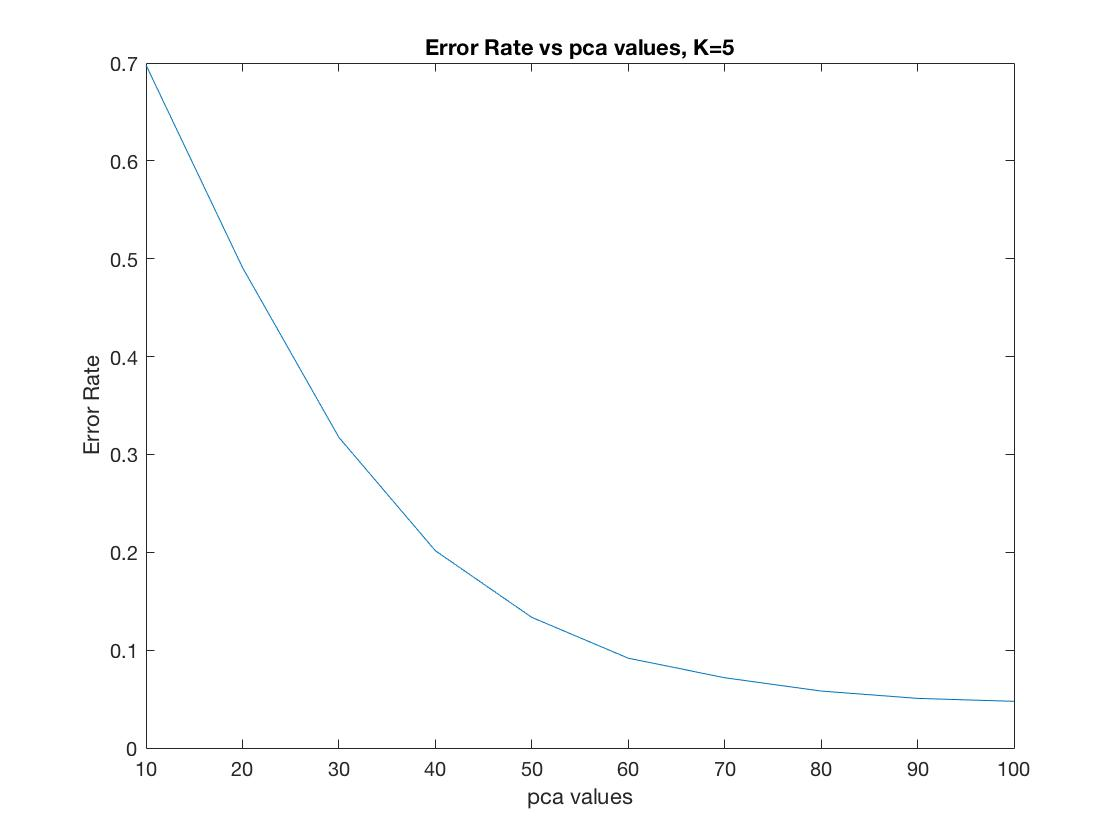
\includegraphics[scale = 0.4]{e121.jpg}\\
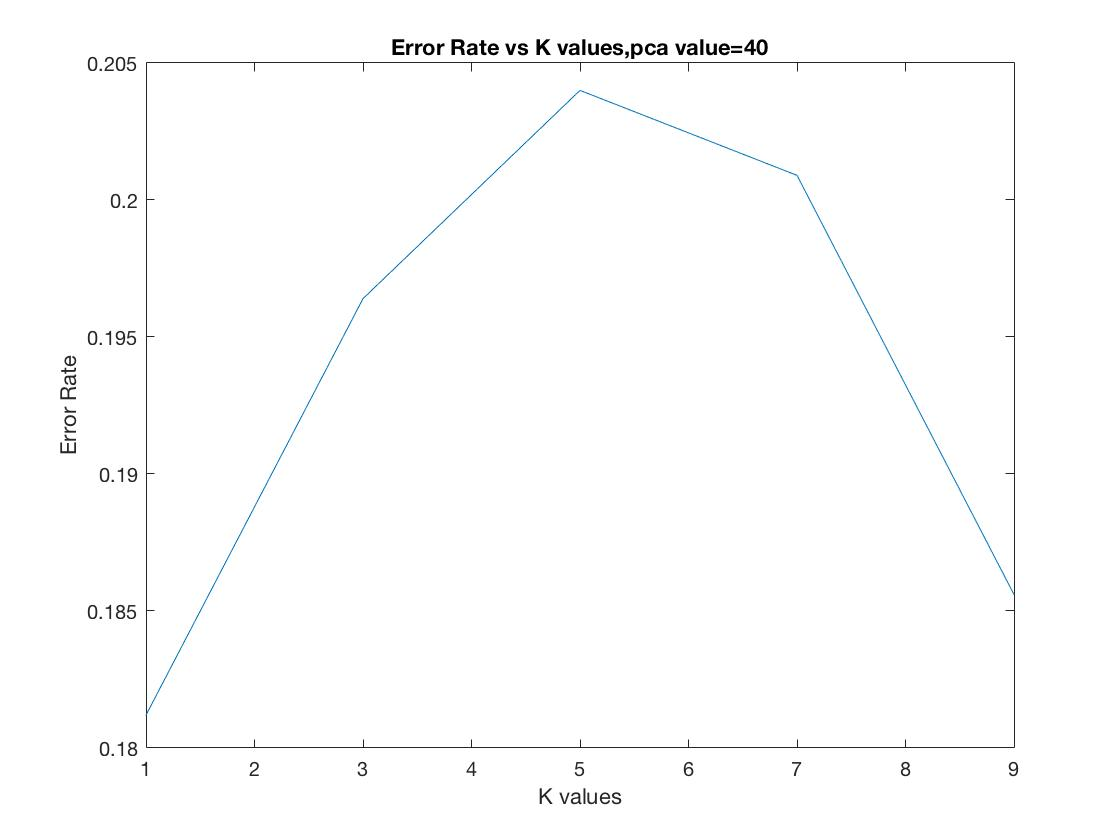
\includegraphics[scale = 0.4]{e122.jpg}\\\\
When I was tuning my parameters ($K$ and $pca\_ value$), when $K=5$, $pca\_ value = 100$, the error rate has reached 4.67$\%$.\\\\


\section{Question 2}
\subsection{Question 2a}
To predict $Z_{t_{n+1}}\mid Z_{t_{1}},Z_{t_{2}},...,Z_{t_{n-1}},Z_{t_{n}}$,
given the fact that\\\\
For a joint Gaussian Distribution $\mathcal{N}(\mu,K)$\\\\
\centerline{$\mu = 
\begin{pmatrix}
  \mu_{1} \\
 \mu_{2}
 \end{pmatrix}$,
 $K = 
\begin{bmatrix}
  K_{11} & K_{12} \\
 K_{21} & K_{22}
 \end{bmatrix}$}
 \\\\
 Where $\mu_{1}$ is the mean vector of $Z_{t_{1}}, Z_{t_{2}}.... Z_{t_{n}}$, $\mu_{2}$ is the mean vector of $Z_{t_{n+1}}$. And $K_{11}$ is the covariance matrix of $Z_{t_{1}} ... Z_{t_{n}}$, $K_{12}$ is the covariance matrix of $Z_{t_{1}} ... Z_{t_{n}}, Z_{t_{n+1}}$, $K_{22}$ is the variance matrix of $Z_{t_{n+1}}$.\\\\
Then the conditional distribution of $Z_{t_{n+1}}$ is\\\\
\centerline{$\mathcal{N}(\mu',K')$}\\\\
Where\\\\
\centerline{$\mu'$ = $\mu_{2}+K_{21}K_{11}^{-1}(Z-\mu_{1}),K'=K_{22}-K_{21}K_{11}^{-1}K_{12}$, $Z = (Z_{t_{1}} ... Z_{t_{n}})$}
\subsection{Question 2b}
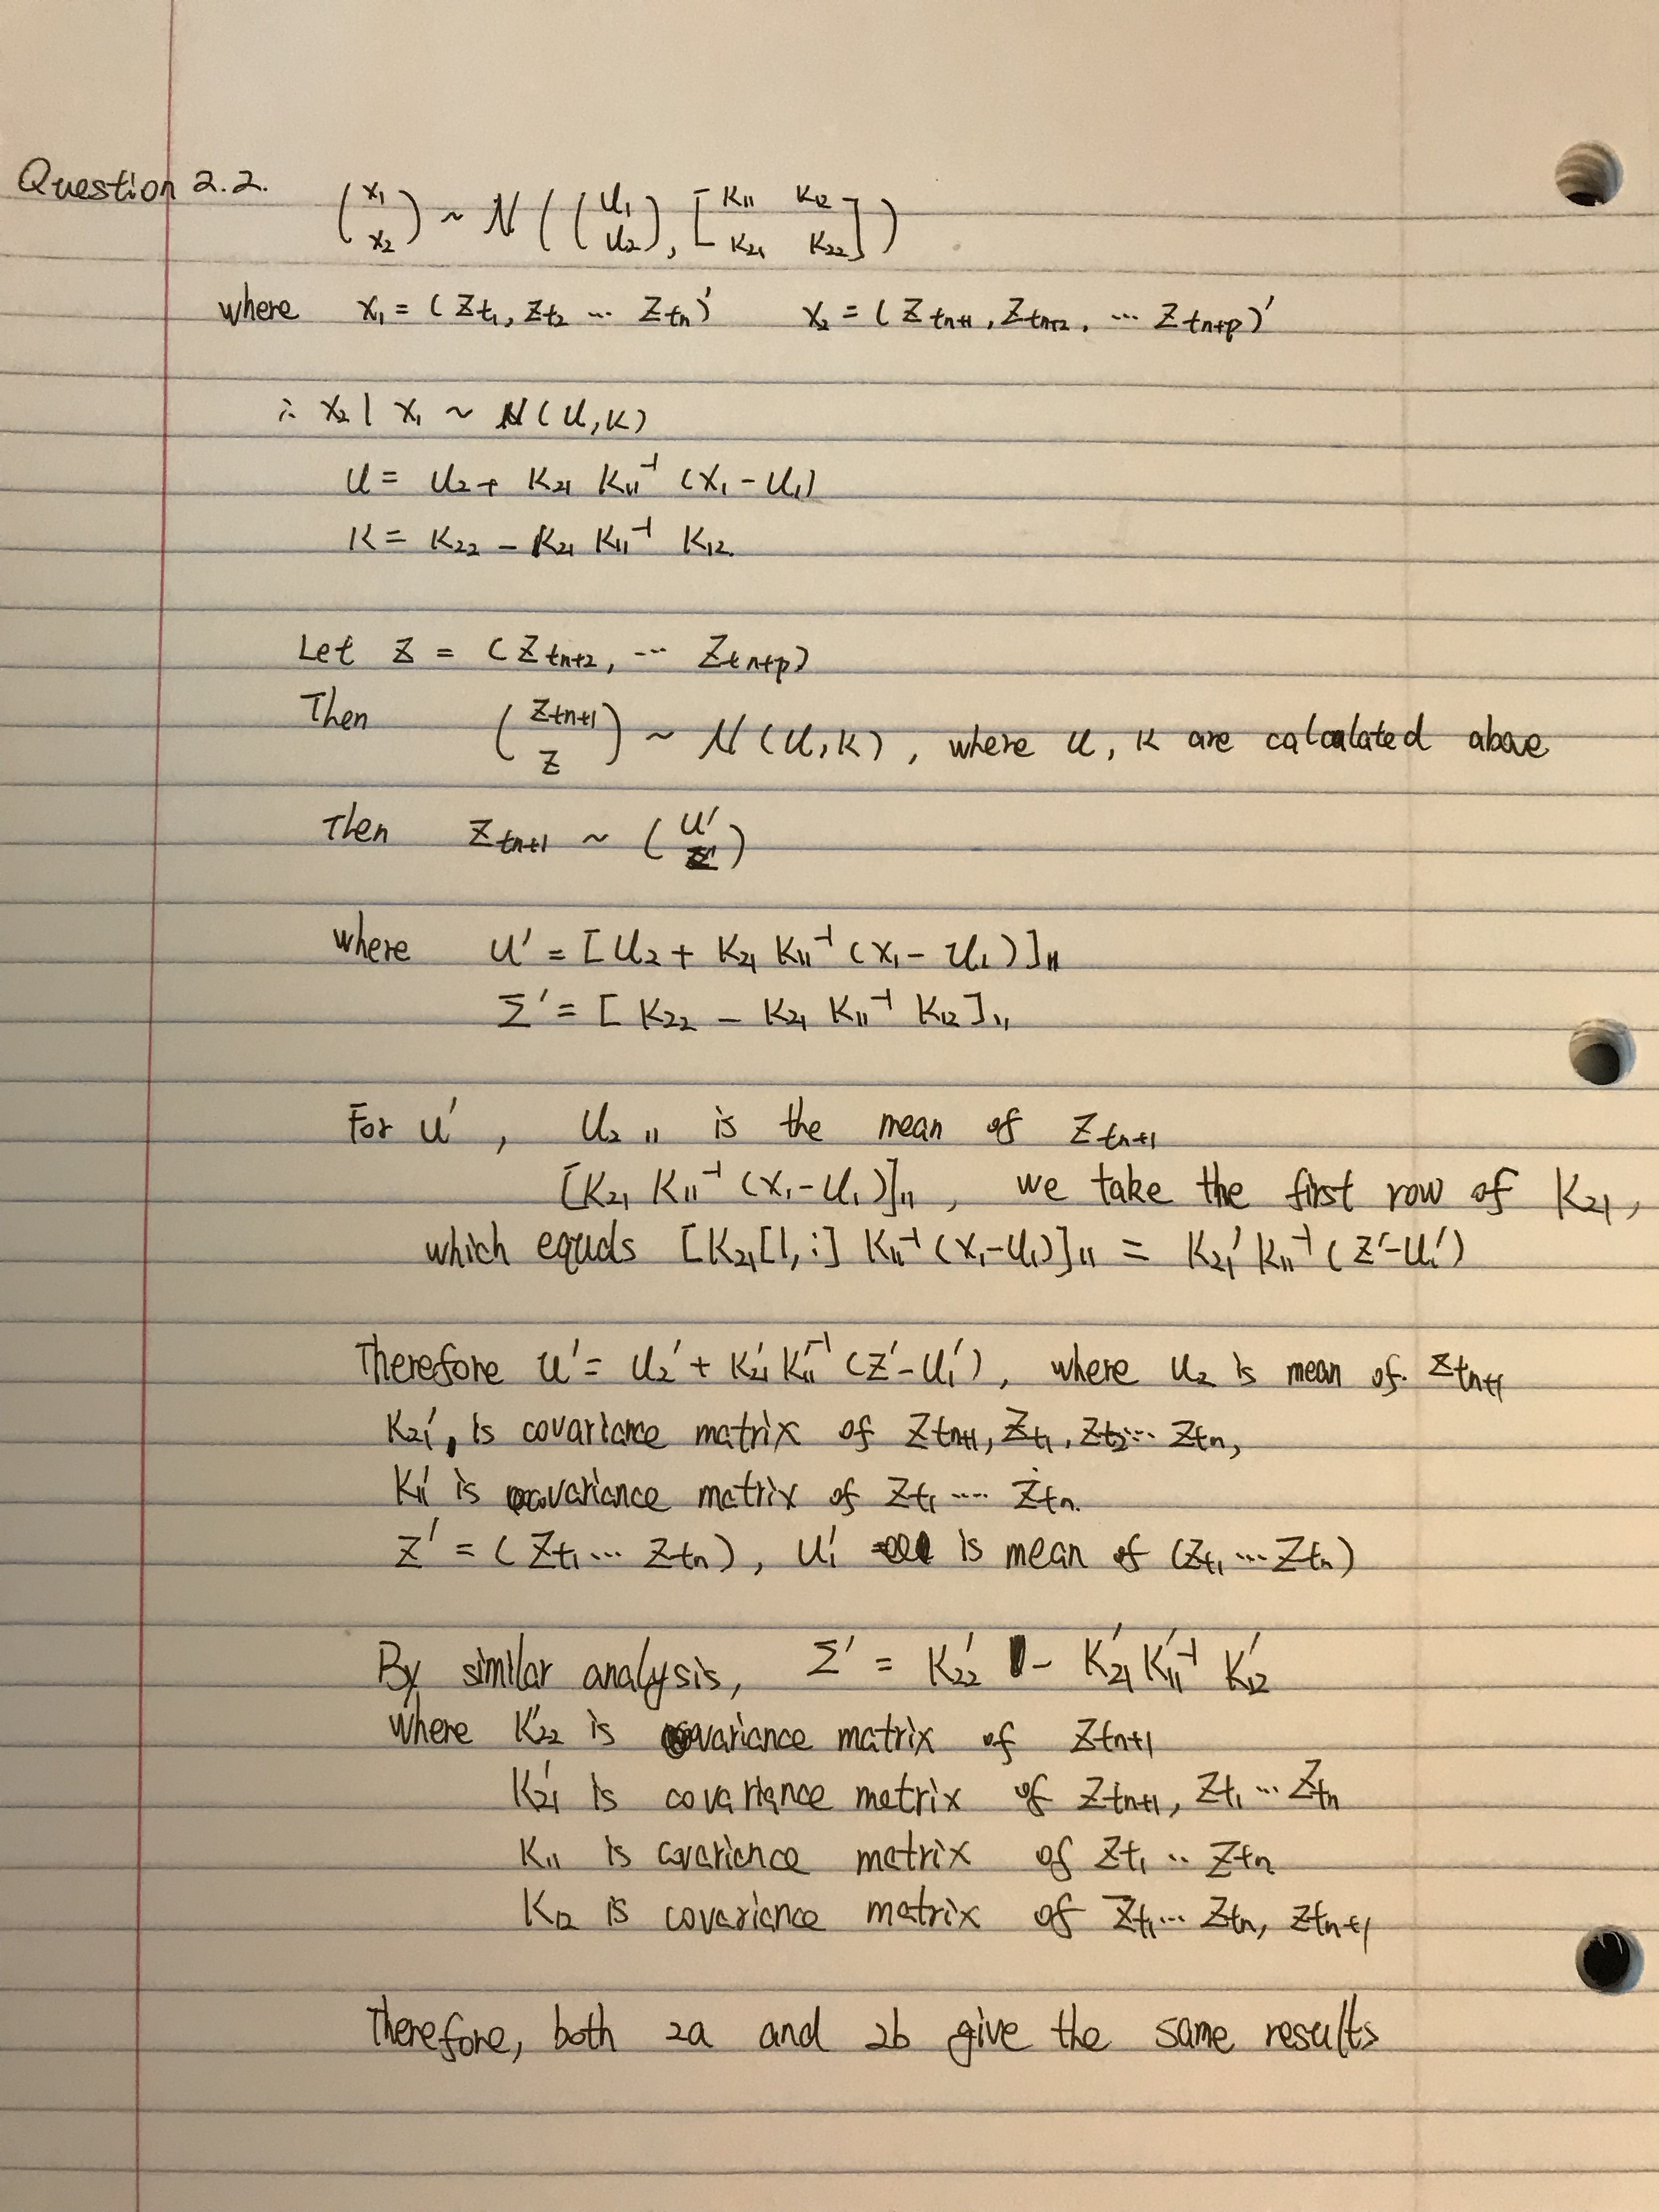
\includegraphics[scale = 0.15]{e22.jpeg}\\
\section{Question 3}
\subsection{Question 3a}
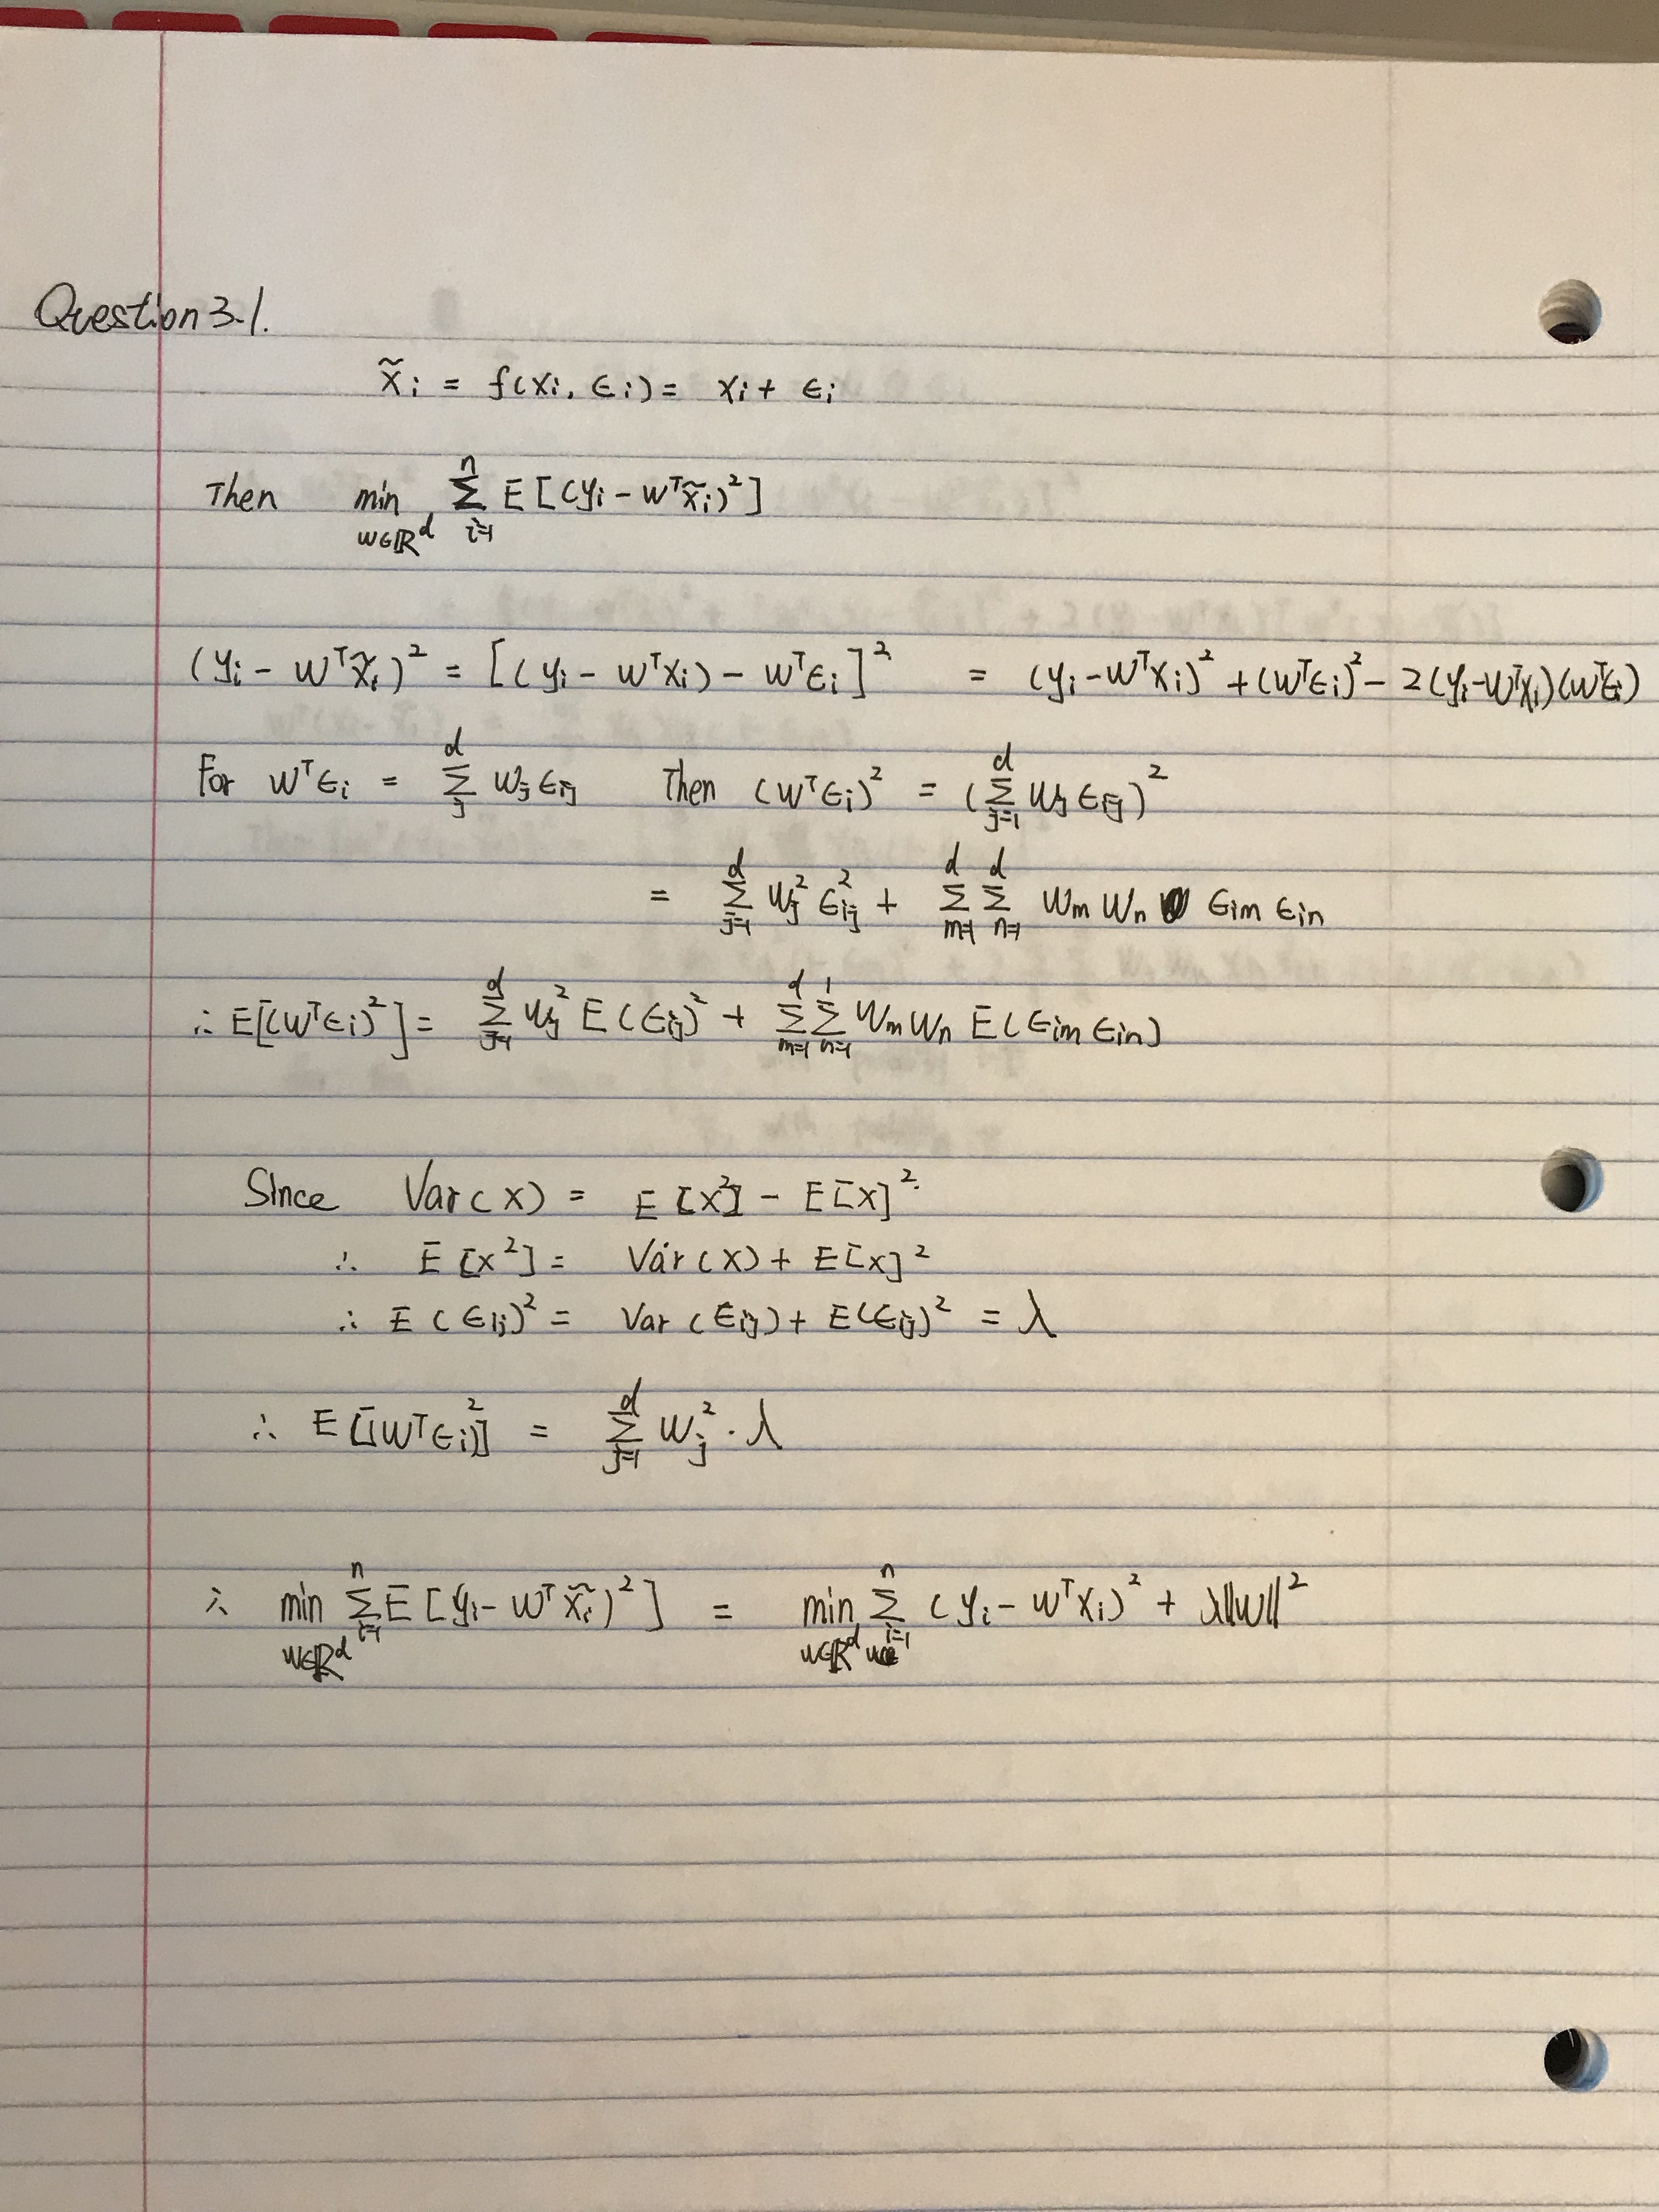
\includegraphics[scale = 0.15]{e31.jpeg}\\

\subsection{Question 3b}
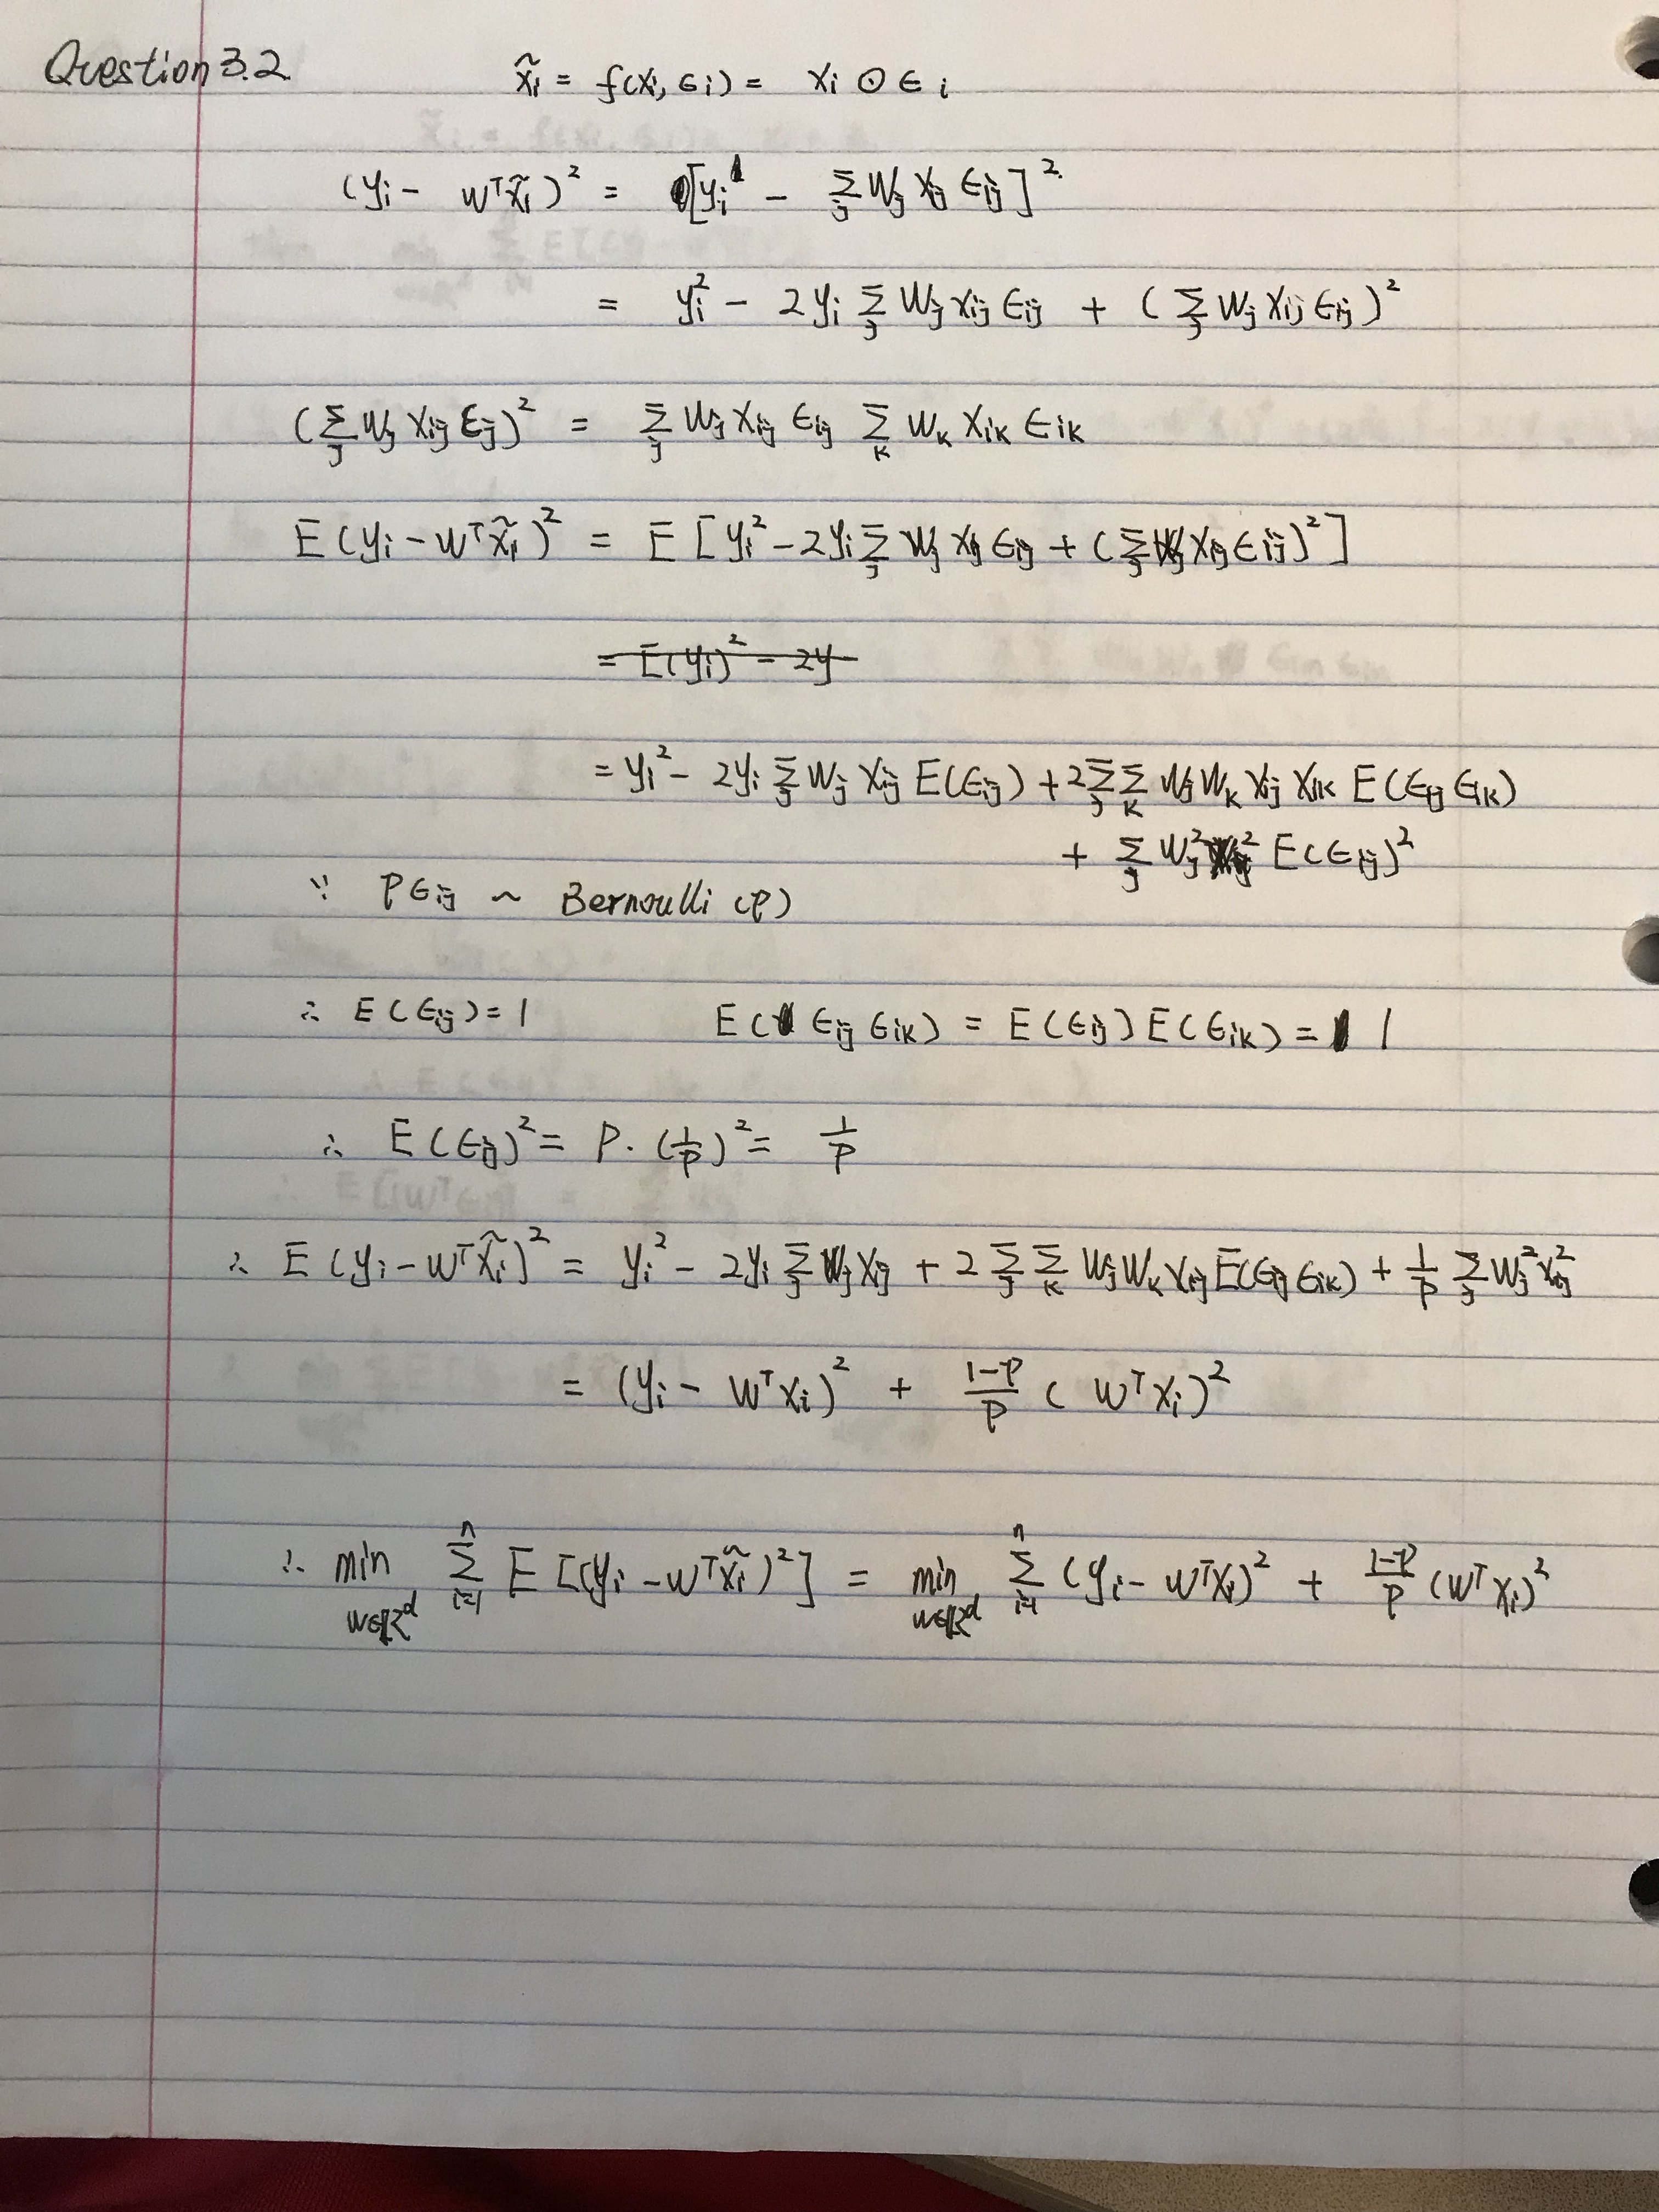
\includegraphics[scale = 0.15]{e32.jpeg}\\


\end{document}
